\section{Methods}

The \soft{HALFpipe} software is containerized, similar to \soft{fMRIPrep}
or \soft{C-PAC}. This means that it comes bundled with all other software
that is needed for it to run, such as \soft{fMRIPrep}
\parencite{10.1038/s41592-018-0235-4}, \soft{MRIQC}
\parencite{10.1371/journal.pone.0184661}, \soft{FSL}
\parencite{10.1016/j.neuroimage.2011.09.015}, \soft{ANTs}
\parencite{10.1016/j.neuroimage.2010.09.025}, FreeSurfer
\parencite{10.1073/pnas.200033797}, and \soft{AFNI}
\parencite{10.1006/cbmr.1996.0014,cox_afni_1997}.
As such, all users of one version of \soft{HALFpipe} will be using the
exact same versions of these tools, because they come with the container.
Thus, the containerization of \soft{HALFpipe} software aids reproducibility
across different researchers and computing environments. We have provided
the \soft{HALFpipe} application in a Singularity container and a Docker
container. Singularity or Docker, which are both freely available, must be
installed prior to downloading the containerized \soft{HALFpipe}
application. Both Docker and Singularity perform so-called
operating-system-level virtualization, but are more efficient and require
less resources than virtual machines. Running Docker containers on a Linux
or macOS operating system requires administrator privileges. Singularity is
typically run on a Linux operating system and may be used without
administrator privileges.

Besides containers, our \soft{HALFpipe} development team adopted other
software engineering best practices, which promoted faster development and
reduced code errors. These industry best-practices, which have found their
way into research applications \parencite{das_programming_2018}, involve
writing code that is easy to read (albeit generally harder to write), the
breakdown of complex systems into several simpler subsystems, dedicated
effort toward thoughtful code design before implementation, and performing
continuous integration via unit tests \parencite{beckkent2000epe:}. The
\soft{HALFpipe} development team applied these practices whenever possible.

\soft{HALFpipe} is being developed as an open-source project and is
accepting contributions that offer new features, enhance functionality, or
improve efficiency. All changes will be reviewed manually. Additionally,
before inclusion in the source tree, changes will undergo automated (unit)
testing, which includes running an entire analysis for one subject of the
OpenNeuro dataset ds000108 \parencite{10.1016/j.neuron.2008.09.006}. This way,
unexpected side effects and bugs can be caught and corrected before causing
problems for users.

\subsection{Databases}

To automatically construct a neuroimaging processing workflow, the program
needs to be able to fulfill queries such as \pseudocode{``retrieve the
structural image for subject x''}. Many programs implement such queries using
a database system. 

For example, the Python implementation of the BIDS
standard, called \soft{PyBIDS}, uses an SQL database on the back-end. Each
file of a BIDS dataset is assigned a number of tags in the database, such
as \code{subject}, \code{task}, or \code{session} to facilitate executing
queries on these tags. The PyBIDS equivalent of the example above would be
\code{layout.get(datatype='anat', sub='x')}. The database approach adds a
layer of complexity, because the database must be defined and populated and
code must be written to interface with the database. For \soft{HALFpipe},
we chose to construct indices and query functions based on native Python
data types.

A further challenge is generating database queries that flexibly interface
with the logic of neuroimaging and processing pipelines, which is relevant
in the context of missing data. \soft{HALFpipe} always tries to execute the
best possible processing pipeline based on the data that is available. For
example, a field map may have been routinely acquired before each
functional scan in a particular dataset. If one of these field maps is
missing, \soft{HALFpipe} flexibly assigns another field map, for example
one belonging to the preceding functional scan. However, \soft{HALFpipe}
will not use a field map from another scan session, as field
inhomogeneities are likely to have changed. Finally, \soft{HALFpipe} does
not fail if a field map is missing, but simply omits the distortion
correction step for that subject. Other examples include the ability of
\soft{HALFpipe} to match structural to functional images, and match task
events to a functional scan. This strategy is used throughout the
construction of processing workflows.

\subsection{Metadata}

Processing of neuroimaging data requires access to relevant metadata, such
as temporal resolution, spatial resolution, and many others. Some elements
of metadata, such as echo time (TE), are represented differently depending
on scanner manufacturer and DICOM conversion software. The method for
reading various types of data has been harmonized in \soft{HALFpipe} using
the following three methods.

First, metadata can be stored in BIDS format. This means that a JavaScript
Object Notation (JSON) file accompanies each image file, which contains the
necessary metadata. BIDS calls this file the \term{sidecar}, and common
tools such as \soft{heudiconv} \parencite{yaroslav_halchenko_2018_1306159} or
\soft{dcm2niix} \parencite{10.1016/j.jneumeth.2016.03.001} generate these files
automatically. If these files are present, \soft{HALFpipe} will detect and
use them. Second, instead of sidecar files, some software tools store image
metadata in the NIfTI header. The NIfTI format defines fields that can fit
metadata, but depending on how the image file was created, these metadata
may be missing. Some conversion programs also place the metadata in the
description field in free text format. This description can also be parsed
and read automatically. Third, information may be incorrectly represented
due to user error, incompatible units of measurement, or archaic technical
considerations. In such cases, \soft{HALFpipe} provides a mechanism to
override the incorrect values. For every metadata field, the user interface
will prompt the user to confirm that metadata values have been read or
inferred correctly. The user can choose to manually enter the correct
values.

\subsection{Interfaces}

\soft{HALFpipe} consists of different modules that need to pass data
between each other, such as file pathnames and the results of quality
assessment procedures. Developing an application as large and complex as
\soft{HALFpipe} requires establishing predictable interfaces, which
prescribe data formats for communication within the application. An
advantage of this approach is that knowledgeable users can write their own
code to interface with \soft{HALFpipe}.

\soft{HALFpipe} uses the Python module \soft{marshmallow} to implement
interfaces, called schemas in the module's nomenclature. All schemas are
defined in the \soft{HALFpipe} code. When the user first starts the
application, the user interface is displayed by \soft{HALFpipe}. It asks
the user a series of questions about the data set and the analysis plan,
and stores the inputs in a configuration file called \filename{spec.json}. The
configuration file has a predictable syntax and can be easily scripted or
modified, which enables collaborative studies to harmonize analysis plans.
\subsection{Workflow engine}

To obtain reproducible results, a core requirement for \soft{HALFpipe} was
reproducible execution of the processing pipeline. As the ENIGMA consortium
requires fMRI analysis of large datasets with several thousand samples,
\soft{HALFpipe} was designed to parallelize processing on multiple
computers or processor cores. Both of these specifications were achieved by
implementation in \soft{Nipype}, \term{NeuroImaging in Python: Pipelines
and Interfaces} \parencite{10.3389/fninf.2011.00013}. \soft{Nipype} is a
workflow engine for neuroimaging that constructs an acyclic directed graph,
in which nodes represent processing commands that need to be executed (the
steps of the pipeline), while the edges represent inputs and outputs being
passed between nodes (images or text files). In this formalization of a
neuroimaging pipeline as a graph, the fastest order for execution across
multiple processor cores can be determined.

The workflow graphs are modular and scalable, which means they can be
nested and extended. \soft{HALFpipe} uses the workflows defined by
\soft{fMRIPrep} and then connects their outputs to additional workflows.
\soft{fMRIPrep} itself is modular and divided into multiple workflows:
\soft{sMRIPrep} \parencite{esteban_oscar_2021_4593442}, \soft{SDCFlows}, and
\soft{NiWorkflows}. The workflow graph facilitates saving and verifying
intermediate results, and supports the user's ability to stop and later
restart processing. \soft{HALFpipe} also uses the graphs to determine which
intermediate results files are not needed by subsequent commands by using a
tracing garbage collection algorithm \parencite{10.1145/359642.359655}. As
such, intermediate files do not accumulate on the storage device. This
feature is implemented as a plugin to \soft{Nipype}.

\soft{Nipype} forms the basis of \soft{fMRIPrep} and \soft{C-PAC}, which
are widely used in the neuroimaging community. However, it has several
limitations that are relevant in the context of \soft{HALFpipe}.
\soft{HALFpipe} is able to calculate features and statistical maps with
different variations of preprocessing settings. To do this efficiently,
intermediate results need to be re-used whenever possible. An improved
second version of \soft{Nipype} is currently being developed, called
\soft{Pydra} \parencite{pydra-proc-scipy-2020}, which will be able to
automatically detect repetitive processing commands, and automatically
re-use outputs. Presently, until \soft{Pydra} becomes available,
\soft{HALFpipe} calculates a four-letter hash code that uniquely identifies
each preprocessing step. Before constructing a new preprocessing command,
\soft{HALFpipe} checks whether its hash has already been added to the
graph. If present, the existing command is re-used.

A key requirement of \soft{HALFpipe} was robust and flexible handling of
missing data. For instance a missing functional scan or statistical map
does not cause \soft{HALFpipe} to fail. Additionally, \soft{HALFpipe}
defines inclusion and exclusion criteria for scans, such as the maximum
allowed motion (mean framewise displacement) or a minimum brain coverage
when extracting a brain region's average signal. Finally, depending on the
data set, statistical maps may need to be aggregated across runs or
sessions within single subjects before a group-level model can be run. This
means that the static graph has to be modified dynamically to adapt to the
results of processing. \soft{HALFpipe} solves this problem by defining a
data structure that not only contains the file names of statistical maps,
but also the tags and metadata that can be used to adjust processing on the
fly. For example, using this data structure, design matrices can be
constructed for group models based on the actual subjects that have
statistical maps available.

\subsection{Running on a high-performance cluster}

\soft{HALFpipe} provides a simple way to run on a high-performance compute
cluster. For each subject, preprocessing and feature extraction takes 6 to
10 hours on a single processor core. Most jobs take about 8 GB to 20 GB of
RAM, depending on size of the data. Assuming each subject is assigned to a
unique job, we recommend requesting 24 GB of RAM for each job. The most
memory-intensive steps of processing are spatial registration and
resampling, and running \soft{FSL MELODIC} for independent component
analysis (ICA) as part of \soft{ICA-AROMA}
\parencite{10.1016/j.neuroimage.2015.02.064}. For large datasets, parallel
processing of subjects is highly desirable to reduce the total computation
time.

Deploying \soft{Nipype} to perform computations on multiple nodes, such as
on a high performance cluster (HPC) is particularly challenging. By
default, \soft{Nipype} submits a separate job to the cluster queue for each
processing command (graph node) regardless of the amount of time required
to execute the command. A watcher process running on the head node collects
outputs from completed commands and submits the next processing command.
This process can be inefficient on some HPCs because computational
resources need to be allocated and deallocated continually. We implemented
a more efficient approach for \soft{HALFpipe} that partitions the
processing graph into many independent subgraphs, which the user may submit
as separate jobs. The smallest granularity available is one subgraph per
subject that is invoked with the command line flag \code{--subject-chunks}.
A \soft{Nipype} workflow is created and validated for all subjects before
the pipeline starts running. In a cluster setting, the most efficient
resource utilization is to submit each subject as a separate job and to run
each job on two CPU cores.

\subsection{Data denoising}\label{sec:denoising}

\soft{HALFpipe} and \soft{fMRIPrep} are modular preprocessing pipelines,
meaning that they utilize a series of tools from various software
libraries. Most have been adopted as standard practice by the community for
many years. Thus, the reasons motivating specific algorithmic choices may
not be readily apparent to users, but need to be considered when designing
tools such as \soft{HALFpipe}. Here we articulate the design considerations
in our selection of tools.

\soft{HALFpipe} performs all denoising in a predefined order after
resampling the fMRI data to standard space using \soft{fMRIPrep}.
\soft{HALFpipe} defines standard space as the \term{MNI152NLin2009cAsym}
template, which is the most current and detailed template available
\parencite{horn_blog}.

\soft{fMRIPrep} not only outputs a preprocessed image in standard space,
but also a spreadsheet with nuisance (or confound) time series. These
include (derivatives of) motion parameters (squared), aCompCor components
\parencite{10.1016/j.neuroimage.2007.04.042}, white matter signal, CSF signal,
and global signal. A key consideration is that including these time series
as nuisance regressors may re-introduce variance that was already removed
in previous processing steps \parencite{10.1016/j.neuroimage.2013.05.116}. An
example of this phenomenon may be regressing out motion parameters after
removing low-frequency drift via temporal filtering. In practice, this
means setting up a regression model for each voxel, where the temporally
filtered time series of a voxel is the dependent variable and the
regressors are the motion parameters. The regression model will calculate a
regression weight for each motion regressor, so that the total model
explains the maximum amount of variance (under assumption of normality).
After multiplying the motion parameters with these weights, they are summed
to yield one time series containing the motion-related noise. This time
series is subtracted from the temporally filtered voxel time series to
yield the result of the procedure, the denoised time series (i.e., the
regression residuals). However, if the motion parameters happen to contain
any low-frequency drift, then their weighted sum likely will as well. It
follows that subtracting a time series with temporal drift from the
temporally filtered voxel data will introduce temporal drift again,
independent of whether a temporal filter was applied before. In
\soft{HALFpipe}, any filter or transformation applied to the voxel time
series is also applied to the nuisance time series. This way, previously
removed variance is not re-introduced accidentally, because it has been
removed from both sides of the regression equation. In \soft{HALFpipe},
denoising is implemented as follows:

\begin{enumerate}[leftmargin=*]

\item

\soft{ICA-AROMA} noise component classification
\parencite{10.1016/j.neuroimage.2015.02.064} relies on reference masks defined
in \term{MNI152NLin6Asym} space, which is different from the standard space
template used by \soft{fMRIPrep}. To solve this issue, \soft{fMRIPrep} will
estimate a second normalization to this template, apply it to the fMRI
image in native space, and run \soft{ICA-AROMA} on the resulting image
\parencite{10.1101/2021.02.10.430678}. This approach effectively doubles the
processor time spent on spatial normalization, and may require manually
checking both spatial registrations. To avoid this considerable effort,
\soft{HALFpipe} resamples the image to \term{MNI152NLin6Asym} space using
an existing transformation/warp field between the two spaces
\parencite{horn_transform}. Specifically, this predefined warp field is
concatenated with the subject's warp to \term{MNI152NLin2009cAsym} space,
with which resampling is performed with \soft{fMRIPrep}'s
\code{bold\_std\_trans\_wf} workflow. Finally, \soft{ICA-AROMA} is run on the
resulting fMRI image in \term{MNI152NLin6Asym} space using
\soft{fMRIPrep}'s \code{ica\_aroma\_wf} workflow, which also includes spatial
smoothing fixed to a 6 mm FWHM smoothing kernel
\parencite{10.1016/j.neuroimage.2015.02.064}. \soft{ICA-AROMA} generates a set
of component time series and a binary classification of these components as
either signal or noise.

\item

\soft{HALFpipe} implements spatial smoothing using \soft{AFNI}'s
\soft{3dBlurInMask} \parencite{10.1006/cbmr.1996.0014}. Each voxel's signal is
averaged with the signal of its neighboring voxels, weighted by an
isotropic gaussian kernel. At the edges of the brain, this kernel may
include non-brain voxels, so smoothing is constrained to only happen within
the brain mask. This is equivalent to the procedure in the \term{Minimal
Preprocessing Pipelines for the Human Connectome Project}
\parencite{10.1016/j.neuroimage.2013.04.127}.

\item\label{itm:grandmean}

Grand mean scaling sets the image mean, defined as the within-scan mean
across all voxels and time points, to a predefined value. The grand mean is
closely related to scanner parameters such as amplifier gain but not to
neural mechanisms \parencite{10.1006/nimg.2002.1226}. Adjusting the grand mean
via scaling makes analysis results more interpretable and comparable across
subjects, sessions, and sites. The scaling factor is calculated based on
the masked functional image, and applied to both the fMRI data and the
nuisance time series extracted by \soft{fMRIPrep}.

\item\label{itm:aroma}

The previously estimated \soft{ICA-AROMA} noise components are removed from
the smoothed and grand-mean-scaled fMRI data. This is done in a
non-aggressive way to minimize removing variance that is shared between
signal and noise components. ICA-AROMA implements this step using the \soft{FSL}
command \soft{fsl\_regfilt}, which calculates an ordinary least squares
regression for each voxel, where the design matrix includes both the signal
and the noise components as regressors. This means that the resulting
regression weights reflect the unique variance of the noise components (and
not the shared variance with signal components). Then, the noise component
regressors are multiplied by their regression weights and added together to
yield one time series of all the noise. Subtracting the noise from the
voxel time series yields a denoised time series (the regression residuals);
this step is done using a re-implementation of \soft{fsl\_regfilt} in
\soft{Numpy} \parencite{10.1038/s41586-020-2649-2}. The same procedure is
applied to the nuisance time series from step~\ref{itm:grandmean}.

\item\label{itm:tempfilt}

Temporal filtering can be used to remove low-frequency drift via a
high-pass filter, high-frequency noise via a low-pass filter, or both at
the same time using a band-pass filter. \soft{HALFpipe} implements two
approaches to temporal filtering, a frequency-based approach
\parencite{10.1155/2013/935154} and a Gaussian-weighted approach
\parencite{10.1006/nimg.2000.0628}. The frequency-based temporal filter is very
exact in selecting frequencies to be kept or removed, and is commonly used
to calculate fractional Amplitude of Low Frequency Fluctuations (fALFF) and
Regional Homogeneity (ReHo). The Gaussian-weighted temporal filter is the
default used by \soft{FSL Feat} \parencite{10.1016/j.neuroimage.2011.09.015}
and may have fewer edge effects at the start and end of the time series.
However, its spectrum also has a more gradual roll-off, meaning that it
will be less aggressive in removing frequencies close to the chosen cutoff
value. Temporal filtering is applied to both the fMRI data and nuisance
time series from step~\ref{itm:aroma}.

\item

Nuisance time series from step~\ref{itm:tempfilt} are removed using the
regression residualization procedure described above from both the fMRI
data and the nuisance time series.

\end{enumerate}

\soft{HALFpipe} suggests default settings for each of these steps, which
are outlined in Table~\ref{table:settings}. Note that some are selected based on
best-practices in the field (i.e., band-pass temporal filter for ALFF and
ReHo), whereas most default settings can be adjusted by the user.

\begin{figure}[!tb]
\begin{adjustwidth}{-2.4cm}{}
\hsize=\linewidth%
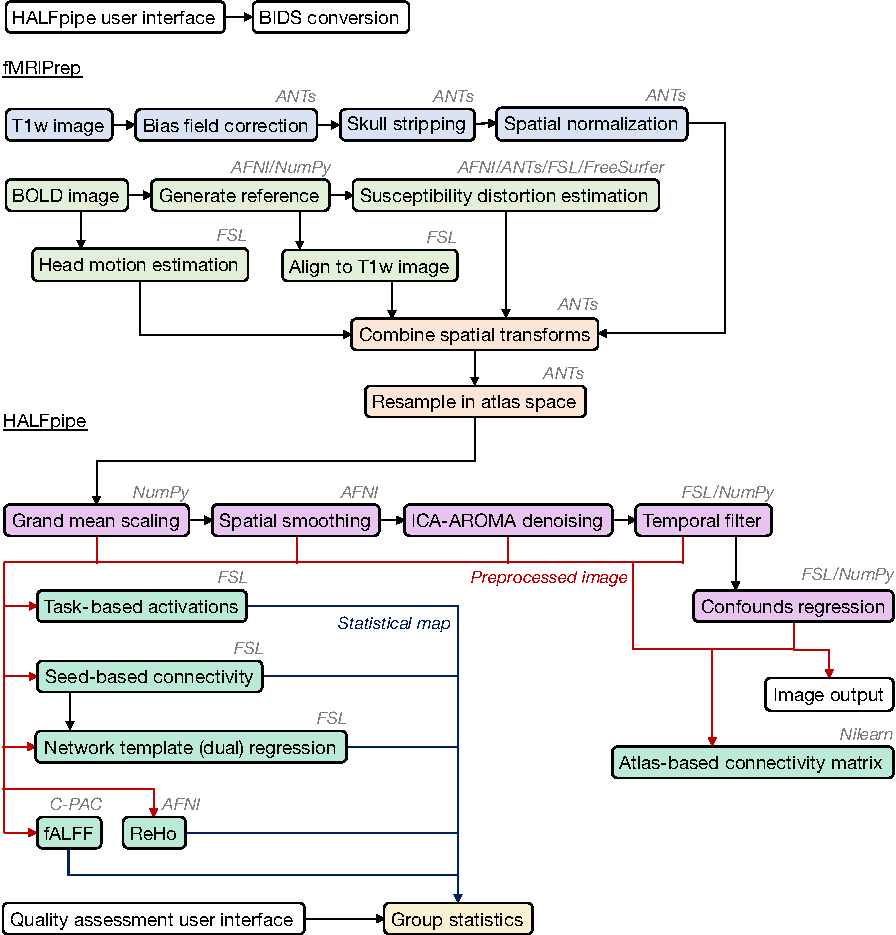
\includegraphics[width=\linewidth]{fig/workflow-crop}
\caption{\textbf{HALFpipe workflow.} After minimal preprocessing with
fMRIPrep \parencite{10.1038/s41592-018-0235-4}, additional preprocessing
steps can be selected (purple). Using the preprocessed data, statistical
maps can be calculated during feature extraction (turquoise). Note that
not all preprocessing steps are available for each feature, as is outlined
in Table~\ref{table:settings}. The diagram omits this information to 
increase visual clarity.}\label{fig:workflow}
\end{adjustwidth}
\end{figure}

\subsection{Quality assessment}\label{sec:qamethods}

Assessing the quality of data and preprocessing is a laborious undertaking
and often done manually. Efforts to automate this process, either through
predefined thresholds of image quality features
\parencite{10.1016/j.neuroimage.2017.10.034} or machine learning
\parencite{10.1371/journal.pone.0184661} are not yet ready to replace the eyes
of a trained researcher checking the data. However, various approaches make
this process easier. First, rather than viewing three-dimensional
neuroimaging files directly, generating and viewing reports containing
two-dimensional images offers a significant time savings. Second, tools
such as \soft{slicesdir} (in \soft{FSL}), \soft{fMRIPrep}, and \soft{MRIQC}
generate HTML files that contain multiple report images and can be explored
in a web browser. \soft{MRIQC} also provides an interactive widget to rate
the quality of each image \parencite{10.1038/s41597-019-0035-4}.

In \soft{HALFpipe}, we use a fixed set of processing steps for quality
assessment. While \soft{slicesdir} allows the researcher to easily compare
the same image type across different subjects, it cannot be used to
generate reports for all types of images. By contrast,
\soft{fMRIPrep}/\soft{MRIQC} HTML files have a broad range of information
and quality report images included, but one HTML file is always specific to
one subject. As such, examining multiple processing steps in many subjects
can be cumbersome. To overcome these issues, \soft{HALFpipe} provides an
interactive web app that is contained in a single HTML file. The app
dynamically loads reports with images, and can handle datasets up to
thousands of images without a performance penalty. The images can be sorted
both by subject, as is done by \soft{fMRIPrep}/\soft{MRIQC}, or by image
type, as is done in \soft{slicesdir}. Each image can be rated as either
good, uncertain, or bad. Predefined logic automatically converts these
ratings into inclusion/exclusion decisions for \soft{HALFpipe}'s group
statistics. In addition, tagging images as uncertain enables users to
efficiently retrieve and discuss these with a colleague or collaborator,
after which a definitive decision on image quality can be made.

Images can be zoomed by clicking them. For faster operation by advanced
users, rating and navigation are accessible not just via user interface
buttons, but also via keyboard shortcuts based on the WASD keys. Pressing
the A goes back one image and D goes ahead, whereas W, S and X rate an
image as good, uncertain or bad, respectively. The web app offers an
overview chart that indicates subjects preprocessed successfully and
subjects with errors, a chart with quality ratings, and box plots
reflecting the sample distributions for motion, noise components, and
temporal signal-to-noise ratio (tSNR). All three are implemented so that
users can hover over chart elements with their cursor to view
meta-information, such as the subject identifier, and click to navigate to
the associated report images. The HTML file is built as a frameworkless web
app using TypeScript. Source code is available at
\url{https://github.com/HALFpipe/QualityCheck}.

\soft{HALFpipe} shows two report images for each subject on
structural/anatomical processing and four additional images for each type
of functional scan. Detailed explanations may be found in the quality
assessment manual at
\url{https://github.com/HALFpipe/HALFpipe\#quality-checks}.

\begin{enumerate}[leftmargin=*]

\item

T1w skull stripping shows the bias-field corrected anatomical image
overlaid with a red line that outlines the brain mask. The user must check
that no brain regions are missing from the mask, and that portions of the
skull or head are not included in the mask.

\item

T1w spatial normalization shows the anatomical image resampled to standard
space overlaid with a brain atlas in standard space. The user needs to
check whether the regions of the atlas closely match the resampled image.

\item

Echo planar imaging (EPI) tSNR shows the temporal signal-to-noise ratio of
the functional image after preprocessing using \soft{fMRIPrep}. The user
must check that signal recovery is distributed uniformly throughout the
brain, and exclude scans with asymmetry, distortions, localized signal
drop-out, or striping artifacts.

\item

EPI Confounds shows the carpet plot
\parencite{10.1016/j.neuroimage.2016.08.009,10.1016/j.neuroimage.2020.116614}
generated by \soft{fMRIPrep}. A carpet plot is a two-dimensional plot of
time series within a scan, with time on the \emph{x}-axis and voxels on the
\emph{y}-axis. Voxels are grouped into cortical gray matter (blue),
subcortical gray matter (orange), cerebellum (green), and white matter and
cerebrospinal fluid (red). Above the carpet plot are time courses (\emph{x}-axis)
of the magnitude (\emph{y}-axis) of framewise displacement (FD), global signal
(GS), global signal in CSF (GSCSF), global signal in white matter (GSWM),
and DVARS, which is the temporal change in root-mean-square intensity (D being the
temporal derivative of time courses and VARS the root-mean-square variance
over voxels). The user must look for changes in heatmap/intensity in
relation to motion and signal changes above. Abrupt changes in the carpet
plot may correspond to motion spikes, whereas extended signal changes may
indicate acquisition artifacts caused by defective scanner hardware.

\item

EPI ICA-based artifact removal shows the time course of the mean signal
extracted from each ICA-component and its classification as either signal
(green) or noise (red). This figure is generated by \soft{fMRIPrep}. For
each component, there is a spatial map (left), the time series (top right)
and the power spectrum (bottom right). The user must check that components
classified as noise do not contain brain networks or temporal patterns that
are known to be signal.

\item

EPI spatial normalization shows the functional image after preprocessing
using \soft{fMRIPrep} overlaid with a brain atlas in standard space. As
before, the user must check whether the regions of the atlas closely match
the resampled image.

\end{enumerate}

\subsection{Statistics}\label{sec:statistics}

\soft{HALFpipe} uses \soft{FSL} FMRIB Local Analysis of Mixed Effects
(FLAME) \parencite{10.1016/j.neuroimage.2003.12.023} for group statistics,
because it considers the within-subject variance of lower level estimates
in its mixed effects models. In addition, its estimates are conservative,
which means they offer robust control of the false positive rate
\parencite{10.1073/pnas.1602413113}.

A common issue in fMRI studies is that the spatial extent of brain coverage
may differ between subjects. A common choice is to restrict higher-level
statistics to only those voxels that were acquired in every subject.
However, with a large variation in brain coverage, which is to be expected
when pooling multi-cohort data, sizable portions of the brain may
ultimately be excluded from analysis. To circumvent this issue,
\soft{HALFpipe} uses a re-implementation of \soft{FSL}'s \soft{flameo} in
\soft{Numpy} \parencite{10.1038/s41586-020-2649-2}. In this implementation, a
unique design matrix is re-generated for every voxel so that only subjects
who have a measurable value for a given voxel are included. Then the model
is estimated using the FLAME algorithm. This list-wise deletion approach
depends on the assumption that voxels are missing completely at random
(MCAR), meaning that the regressors (and thus statistical values) are
independent of scanner coverage.

For group models, users can specify flexible factorial models that include
covariates and group comparisons. By default, missing values for these
variables are handled by list-wise deletion as well, but the user may
alternatively choose to replace missing values by zero in the demeaned
design matrix. The latter approach is equivalent to imputation by the
sample mean. Design matrices for the flexible factorial models are
generated using the Python module \soft{Patsy}
\parencite{nathaniel_j_smith_2018_1472929}. Contrasts between groups are
specified using the \soft{lsmeans} procedure \parencite{jssv069i01}.

\begin{tablebox}[label={table:settings}]{Default values for preprocessing settings per feature}

\begingroup%
\newcolumntype{L}{>{\raggedright\arraybackslash}X}%
\newcolumntype{C}{>{\centering\arraybackslash}X}%
\newcolumntype{K}[1]{>{\raggedright\arraybackslash}m{#1}}%
\newcolumntype{M}[1]{>{\centering\arraybackslash}m{#1}}%
\renewcommand\tabularxcolumn[1]{m{#1}}%
\renewcommand{\arraystretch}{1.35}%
\begin{tabularx}{\textwidth}{@{} | K{2cm} |
M{1.9cm} | C | C | M{1.4cm} | C | c | c | @{}} 
\hhline{~|-|-|-|-|-|-|-|}
\multicolumn{1}{c|}{} & 
\textbf{Preprocessed image} & 
\textbf{Task-based activation} &
\textbf{Seed-based connectivity} & 
\textbf{Dual regression} &
\textbf{Atlas-based connectivity matrix} & 
\textbf{ReHo} & 
\textbf{fALFF} \\
\hhline{-|-|-|-|-|-|-|-|}
Spatial smoothing &%
\multicolumn{4}{c|}{\cellcolor{leaLightGreen}6 mm} &%
\cellcolor{leaGrey} &%
\multicolumn{2}{c|}{\cellcolor{leaLightGreen}6 mm*} \\
\hhline{-|-|-|-|-|-|-|-|}
Grand mean scaling &%
\multicolumn{7}{c|}{\cellcolor{leaLightGreen}10,000} \\
\hhline{-|-|-|-|-|-|-|-|}
ICA-AROMA &%
\multicolumn{7}{c|}{\cellcolor{leaLightGreen}Yes} \\ [2ex]
\hhline{-|-|-|-|-|-|-|-|}
Temporal filter &%
\multicolumn{4}{c|}{\cellcolor{leaLightGreen}Gaussian (128 s FWHM)} &% 
  \multicolumn{3}{c|}{\cellcolor{leaLightGreen}Frequency-based (0.01--0.1 Hz)} \\ [2ex]
\hhline{-|-|-|-|-|-|-|-|}
Confound removal &%
\cellcolor{leaLightGreen}None &%
\multicolumn{3}{c|}{\cellcolor{leaGrey}} &%
\multicolumn{3}{c|}{\cellcolor{leaLightGreen}None} \\
\hhline{-|-|-|-|-|-|-|-|}
Add confounds to model &%
\cellcolor{leaGrey}&%
\multicolumn{3}{c|}{\cellcolor{leaLightGreen}None} &%
\multicolumn{3}{c|}{\cellcolor{leaGrey}} \\
\hhline{-|-|-|-|-|-|-|-|}
\end{tabularx}\par
\vspace*{2mm}
Note: Cells filled in grey indicate that this option cannot be selected in
the user interface, all other settings can be adapted by the user; * done
on the statistical maps after feature extraction.
\endgroup

\end{tablebox}

